% Created 2019-02-11 Mon 21:56
% Intended LaTeX compiler: pdflatex
\documentclass[11pt]{article}
\usepackage[utf8]{inputenc}
\usepackage[T1]{fontenc}
\usepackage{graphicx}
\usepackage{grffile}
\usepackage{longtable}
\usepackage{wrapfig}
\usepackage{rotating}
\usepackage[normalem]{ulem}
\usepackage{amsmath}
\usepackage{textcomp}
\usepackage{amssymb}
\usepackage{capt-of}
\usepackage{hyperref}
\author{Hassan Shabbir}
\date{\today}
\title{Editing Text With Vim}
\hypersetup{
 pdfauthor={Hassan Shabbir},
 pdftitle={Editing Text With Vim},
 pdfkeywords={},
 pdfsubject={},
 pdfcreator={Emacs 26.1 (Org mode 9.1.14)}, 
 pdflang={English}}
\begin{document}

\maketitle
\tableofcontents

\newpage
\section{The main text editors}
\label{sec:org91c0bff}
There are two main (extensible) text editors for Unix and Gnu/Linux operating
systems. These are the VI and Emacs lines of text editors.

Both of these text editors are highly configurable and therefore are highly
recommended by many programmers.
\subsection{VI}
\label{sec:org9a38c04}
VI (pronounced "ve-eye"), and other text editors based off of it are great at
creating and editing text. It is (usually) a basic text editor, however newer
versions of it allow a user to customize it and get IDE-like features within it.
The main feature of VI is the way in which it allows a user to edit text.
\subsection{Emacs}
\label{sec:org1f6a91e}
Emacs (pronounced "ee-maks") is a text editor that is extremly configurable, and
allows for a lot more IDE-like features. This is due to the fact that Emacs is a
text editor based upon the functional programming language Lisp. This means that
you are able to use a general purpose programming language to modify the text
editor. Emacs can also emulate VI keybindings using EVIL mode (EVIL stands for
Extensible VI Layer).
\subsection{Emacs and VI Lore}
\label{sec:org64bf6e6}
\begin{description}
\item[{Lore:}] a body of traditions and knowledge on a subject or held by a particular group,
typically passed from person to person by word of mouth.
\end{description}

Both of these text editors are really amazing, so much so that since their
inception many programmers have been arguing over which text editor is better,
see \href{https://en.wikipedia.org/wiki/Editor\_war}{The Editor Wars (clickable)}.

VI is the editor of the beast since VI in roman numerals is 6, so VI VI VI would
be 666.

From here on out we will be talking about the VI line of editors. The curious
reader is encouraged to read more about Emacs, if interested.
\section{Which Vim version should I use?}
\label{sec:orgd74e5eb}
NOTE: There is almost no difference between these different text editors except
for the information written below.

NOTE: I will assume that Vim/NeoVim is used for the rest of this file, but will
refer to it as Vim, since I am lazy.

There are three different VI versions you should be familiar with.
\subsection{VI}
\label{sec:org0d894a6}
VI\footnote{VI pronounced "ve-eye", also pronounced "vy" but that is an unofficial pronounciation} is the oldest text editor we will be looking at, which was created
in 1976. VI is short for Visual, differentiating it from line editors.\footnote{Technically, the "ed" and "ex" editors are even older, but they literally
show you nothing (you have to manually print lines), so it is like editing text
in the dark. This is where the command mode in VI comes from, see below. Also see
\href{https://sanctum.geek.nz/arabesque/actually-using-ed/}{Actually Using Ed (clickable)} for some extreme masochism.} If
you plan to work with many servers, you should expect literally expect every
server to have it. It is very minimalistic so it won't tell you when you are in
insert mode in any way (see below), for example. This makes it harder to
understand for beginners, and doesn't have all the features of Vim.
\subsection{Vim}
\label{sec:orgbf6c06f}
Vim\footnote{VIM pronounced "vim"} is the newer version of VI, first released in 1991. Due to it being
very popular for a long time, and still is (last stable release: 17 May 2018),
it has many resources available on the internet for it. It is also recently
modern, so it shouldn't be too difficult to use. Therefore, whenever searching
for general vim resources use vim in the search terms.
\subsection{NeoVim}
\label{sec:org119c1be}
NeoVim\footnote{NeoVim pronounced "neo-vim". The command to run it is \texttt{nvim} NOT \texttt{neovim}, and it
can be installed using \texttt{sudo apt install nvim}.} is the newest version of vim, first released in November 1, 2015.
This has the most interactive features and therefore is the one that I would
recommend to new users. For example, when you switch between different modes,
the cursor changes, helping you to remember which mode you are in.
\section{Modal editing with Vim}
\label{sec:org8d646ad}
The first thing you need to know about Vim is that there are four main modes in
which you operate. Each of these modes change what the keys on your keyboard
will do.

\begin{figure}[htbp]
\centering
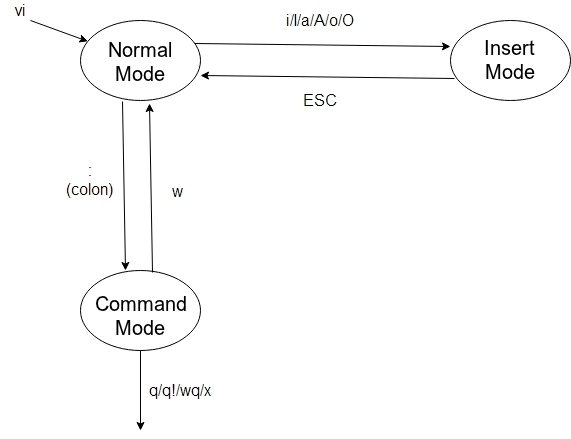
\includegraphics[width=.9\linewidth]{./modes.jpg}
\caption{\label{fig:org7433c09}
Vim Modes, and the way to access different Modes (Modified horribly by me).}
\end{figure}

In general, when editing text you will mostly be making small changes, and very
rarely do you create whole documents without mistakes from start to finish (\texttt{cat
> foo.txt} anyone?). For this reason, Vim is optimized for modifying text.
Understanding modal editing (along with composability, repeatability, and text
objects) is the key to understanding Vim\footnote{For more on how vim works see this awesome answer on Stackoverflow
\href{https://stackoverflow.com/questions/1218390/what-is-your-most-productive-shortcut-with-vim}{Your problem with Vim is that you don't grok vi (clickable).}}.
\subsection{Normal Mode (Movement; Modification)}
\label{sec:org108e319}
Normal mode allows you to issue commands to Vim, which will then do something,
other than putting the key that you pressed into the file. When you first open a
file you will be in Normal Mode. Pressing keys such as \texttt{j} or \texttt{l} will move the
cursor rather than adding those letters to the file. You should almost always be
in Normal Mode, since editing text requires the ability of moving around the
document, and deleting, replacing, copying text, etc. which are all possible in
Normal mode. Thus this mode is called "normal" since it is the default mode when
using Vim. To get back into Normal Mode use the escape key, or control and the
left-squrebracket key.
\subsection{Insert Mode (Add Text)}
\label{sec:orgb5d68c2}
When opening a document with Vim, you will be in Normal Mode. To get into Insert
Mode, you can press keys such as \texttt{i} or \texttt{a} and then you will be in Insert Mode.
If you are using NeoVim, you will see the cursor become thin, and in both Vim
and NeoVim you will see \texttt{-{}-INSERT-{}-} at the bottom of the terminal.\footnote{In VI you will neither see the cursor change nor the \texttt{-{}-INSERT-{}-} at the bottom} You
can then use the arrow keys to get to the location, and press the keys to add
them to the document. To get back to Normal Mode press escape. (This is not
recommended, but can help you get used to Vim. Movement should be done using
Normal Mode, not the arrow keys, allowing your hand to stay on home row) You
will notice that the cursor will become a block again in NeoVim.
\subsection{Command Mode (System Commands; Ed commands)}
\label{sec:org21e5874}
For now, the most important command mode you need to know will be the commands
to exit Vim (which is accessible from Command Mode). This is such a problem for
beginners that \href{https://stackoverflow.com/questions/11828270/how-to-exit-the-vim-editor}{this stackoverflow answer (clickable)} has 4,000 upvotes, and over
1 Million views. The first step is to press \texttt{:} from Normal Mode. If you are not
in Normal Mode, get to it using the escape key. You will now see a colon on the
last line of the terminal. If you wish to save your changes type \texttt{wq}, and then
press enter. This command stands for write (save) the file then quit Vim. If you
wish to throw away your changes type \texttt{q!} and then press enter.
\subsection{Visual Mode (Select Text)}
\label{sec:org3e0c27c}
Visual Mode is used for performing an operation over all of the characters in
the text. This can be useful when you don't know how to run operations using
text objects. Text objects will replace most simple uses of Visual Mode.
\section{Basic Vim editing commands}
\label{sec:orgbbc6b49}
NOTE: Only learn the commands that you want. Then when you get annoyed by
inefficiency come back to learn more.

NOTE: Pressing the Escape key will return you back to Normal Mode from any mode.

NOTE: Vim uses mnemonic devices (ie. \texttt{d} stands for delete) to help you remember
what command does what. Use this to remember what each command does. Also,
commands that are related, but do something different are capitalized, and the
default action is defined by the repeated letter (such as \texttt{dd} for delete with
default action).

Sections will be in the form: CommandName (from StartingMode)

Commands will be in the form:
\begin{itemize}
\item \texttt{COMMAND}: (mnemonic device) Description of command
\end{itemize}
\subsection{Entering Vim (from bash prompt)}
\label{sec:orgf83640d}
You can enter Vim from the commandline (not to be confused with Vim's Command
Mode) by typing \texttt{vim file.txt}, replacing \texttt{file.txt} for the file you want to
edit. If the file doesn't exist, it will be created. You will now be in Vim.
\subsection{Movement Commands (from Normal Mode)}
\label{sec:org5e6eaac}
\subsubsection{Character Movement}
\label{sec:orgb21eb39}
\begin{itemize}
\item \texttt{h}: Move cursor left
\item \texttt{j}: Move cursor down
\item \texttt{k}: Move cursor up
\item \texttt{l}: Move cursor right
\end{itemize}

The way to remember this is that the \texttt{h} key is on the left of the four keys,
\texttt{l} is on the right, \texttt{j} is written with the hook below the line, and \texttt{k} has
the vertical line above the line.

\begin{figure}[htbp]
\centering
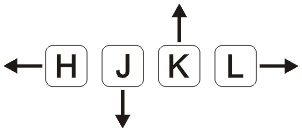
\includegraphics[width=.9\linewidth]{./hjkl.png}
\caption{\label{fig:orge9c37bd}
A graphical depiction of h, j, k, l}
\end{figure}

\subsubsection{Word Movement}
\label{sec:org6eae44f}
\begin{itemize}
\item \texttt{w}: (Word) Go forward by one word
\item \texttt{b}: (Back) Go back by one word
\item \texttt{e}: (End) Go to the next end of word
\end{itemize}

\subsubsection{Line Movement}
\label{sec:org29b50f4}
\begin{itemize}
\item \texttt{\textasciicircum{}}: (This is from Regexes) Go to start of line
\item \texttt{\$}: (This is from Regexes) Go to end of line
\end{itemize}
\subsubsection{File Movement}
\label{sec:orgb976ca5}
\begin{itemize}
\item \texttt{gg}: Go to start of file
\item \texttt{G}: Go to end of file
\end{itemize}

\subsubsection{Find Char Movement}
\label{sec:org7778af2}
\begin{itemize}
\item \texttt{f}: (Find Char) Find character forward
\item \texttt{F}: (Find Char) Find character backward
\item \texttt{;}: Run \texttt{f} / \texttt{F} again
\item \texttt{,}: Run \texttt{f} / \texttt{F} again in opposite direction
\end{itemize}

\subsubsection{Search Term Movement}
\label{sec:org2ab05dc}
\begin{itemize}
\item \texttt{/}: Enter search term, then press enter
\item \texttt{n}: (Next) Go to next location matching search term
\item \texttt{N}: (Previous/Backwards Next) Go to previous location matching search term
\end{itemize}

\subsection{Insert Commands (from Normal Mode)}
\label{sec:orgfc05fd2}
These commands will change you automatically from Normal Mode
to Insert Mode.
\begin{itemize}
\item \texttt{i}: (Insert) Enter Insert Mode before current character
\item \texttt{I}: (Insert) Enter Insert Mode at the beginning of the line
\item \texttt{a}: (Append) Enter Insert Mode after current character
\item \texttt{A}: (Append) Enter Insert Mode at the end of the line
\end{itemize}

\subsection{Deletion Commands (from Normal Mode)}
\label{sec:org97f7faf}
NOTE: The composable nature of Vim should be apparent in this section.

\begin{itemize}
\item \texttt{x}: Delete character under cursor
\item \texttt{dd}: (Delete, Default) Delete current line
\item \texttt{dw}: (Delete Word) Delete until the end of the word
\item \texttt{d3w}: (Delete Word) Delete 3 number of words, etc.
\item \texttt{diw}: (Delete In Word) Delete the whole word
\item \texttt{diw}: (Delete In Word) Delete the whole word
\item \texttt{diW}: (Delete In Word) Delete the whole space delimited word
\end{itemize}
\subsection{Deletion Commands (from Visual Mode)}
\label{sec:orgead8ae7}
\begin{itemize}
\item \texttt{d}: (Delete) Delete current visual selection
\item \texttt{x}: (Delete) Delete current visual selection
\end{itemize}

\subsection{Change Commands (from Normal Mode)}
\label{sec:org2142d7b}
Change deletes something then puts you in Insert Mode
to add text.

\begin{itemize}
\item \texttt{cc}: (Change, Default) Delete line, then go into Insert Mode
\item \texttt{cw}: (Change Word) Delete until the end of the word, then go into Insert Mode
\item \texttt{c3w}: (Change Word) Delete 3 number of words, etc., then go into Insert Mode
\item \texttt{ciw}: (Change In Word) Delete the whole word, then go into Insert Mode
\item \texttt{ciw}: (Change In Word) Delete the whole word, then go into Insert Mode
\item \texttt{ciW}: (Change In Word) Delete the whole space delimited word, then go into Insert Mode
\end{itemize}

\subsection{Yank (Copy) Commands (from Normal Mode)}
\label{sec:orgceeba1c}
NOTE: To copy text to use in other applications, use the \texttt{"+} prefix, see
registers below.

\begin{itemize}
\item \texttt{yy}: (Yank, Default) Yank (copy) the current line, for Vim use only
\item \texttt{yiw}: (Yank) Yank (copy) the current line, for Vim use only

\item \texttt{"+yy}: (Yank, Default) Yank (copy) the current line, for any application
\item \texttt{"+yiw}: (Yank) Yank (copy) the current line, for any application
\end{itemize}
\subsection{Yank (Copy) Commands (from Visual Mode)}
\label{sec:org5127427}
\begin{itemize}
\item \texttt{y}: (Yank) Yank (copy) current visual selection
\end{itemize}
\subsection{Paste Commands (from Normal Mode)}
\label{sec:org15c49b4}
\begin{itemize}
\item \texttt{p}: (Paste) Paste the last deletion/yank
\end{itemize}
\subsection{Paste Commands (from Visual Mode)}
\label{sec:orgc88ae74}
\begin{itemize}
\item \texttt{p}: (Paste) Paste, replacing current visual selection
\end{itemize}
\subsection{Undo Command (from Normal Mode)}
\label{sec:orgbbcc076}
\begin{itemize}
\item \texttt{u}: (Undo) Undo last change
\end{itemize}
\subsection{Visual Mode Commands (from Normal Mode)}
\label{sec:orgb52848e}
First enter Visual Mode using any of the below, then make the selection using
the movement commands as you would from Normal Mode. Then run the command on the
selection, such as yank, delete, etc.

\begin{itemize}
\item \texttt{v}: Enter character-wise Visual Mode
\item \texttt{V}: Enter line-wise Visual Mode
\item \texttt{ctrl-v}: Enter block-wise Visual Mode
\end{itemize}
\subsection{Command Mode (from Normal Mode)}
\label{sec:org504d1cd}
\begin{itemize}
\item \texttt{:w}: Write the file
\item \texttt{:q}: Quit Vim, without having modified the file
\item \texttt{:q!}: Quit Vim, throwing away modifications
\item \texttt{:wq}: Write the file, then quit Vim
\item \texttt{:x}: Shorthand for \texttt{:wq}
\item \texttt{:! date}: Run bash command \texttt{date} and show the result without adding to file
\item \texttt{:r! date}: Run bash command \texttt{date} and read in the result into the file
\end{itemize}
\subsection{Command Mode (from Visual Mode)}
\label{sec:orga6e8057}
Visually select text then enter Command Mode using \texttt{:}. NOTE: you will see
\texttt{:'<,'>} instead. This just tells Vim to run the command over the whole
selection.\footnote{So the command will run in the range \texttt{x,y}, and 
a \texttt{'a} refers to the mark a, with the \texttt{<} referring to the first and \texttt{>}
referring to the last selection. So all together it says "run the command from
the beginning of the selection, to the end of the selection."}

\begin{itemize}
\item \texttt{:'<,'>! wc -l}: Run bash command on visually selected text
\end{itemize}
\section{Composability and Repeatability}
\label{sec:orgfdeb1c2}
\subsection{Text Objects}
\label{sec:org5d2794e}
NOTE: All text objects can be used with delete, yank, copy, etc.

\begin{itemize}
\item \texttt{iw}: (In Word)
\item \texttt{aw}: (All Word)
\item \texttt{is}: (In Sentence)
\item \texttt{as}: (All Sentence)
\item \texttt{ip}: (In Paragraph)
\item \texttt{ap}: (All Paragraph)
\item \texttt{i"}: (In Quote)
\item \texttt{a"}: (All Quote)
\item \texttt{i\}}: (In Brace)
\item \texttt{a\}}: (All Brace)
\item \texttt{it}: (In Tag) Used in HTML
\item \texttt{at}: (All Tag) Used in HTML
\end{itemize}
\subsection{Dot (\texttt{.}) command}
\label{sec:org4ff568c}
The dot command repeats the last complete command that you ran. For example if
you changed a word to "Hi" using \texttt{ciwHi} and then escape, you can change another
word to "Hi" using dot.

This is one way of renaming variables. First search for a variable using \texttt{/},
then using \texttt{ciw} change the variable to something else. Finally, repeat this
change all throughout the document using \texttt{n} to go to the next instance, and \texttt{.}
to run the change.
\subsection{Number Prefixes}
\label{sec:org662f026}
Most commands can be prefixed, meaning you can run commands like \texttt{d5w} which
will delete the next 5 words.
\subsection{Macros}
\label{sec:org8e362a8}
Macros can be used for creating groups of repeatable commands. In other words,
start macro, run general commands (ie. \texttt{w} rather than \texttt{llllllll}), stop macro,
run the macro previously defined on all of the remaining text.

\begin{itemize}
\item \texttt{qa}: Record Macro in register \texttt{a}, see below
\item \texttt{q}: While recording, it will end the macro
\item \texttt{@a}: Run Macro in register \texttt{a}
\end{itemize}
\section{Registers}
\label{sec:org7c462b6}
The most important part about registers is that the \texttt{"+} register is used to
store the global clipboard, which can be accessed by any program. Frankly, I
don't use registers at all otherwise.
\section{Extending Vim for yourself}
\label{sec:orgca167bd}
To change the default behaviour of Vim, you can modify a configuration file
called \texttt{.vimrc} (in Gnu/Linux) or \texttt{\_vimrc} (in Windows, I think).

This will allow you to use plugins, change colorshemes, map keys to commands,
etc.

\subsection{Plugins}
\label{sec:org6d0c83c}
These are a few plugins that I would consider quite useful. All links clickable.

\begin{itemize}
\item \href{https://github.com/junegunn/vim-plug}{Vim Plug}: Vim plugin manager
\end{itemize}
To be able to use the below plugins you need to install a plugin manager, this
is the one I personally use.

\begin{itemize}
\item \href{https://github.com/tpope/vim-sensible}{Vim Sensible}: default settings for Vim
\end{itemize}
This is useful for starting off in Vim. (Not needed for NeoVim.)

\begin{itemize}
\item \href{https://www.github.com/tpope/vim-commentary}{Vim Commentary}: (un)comment lines of code
\item \href{https://www.github.com/tpope/vim-surround}{Vim Surround}: surround text objects with text
\item \href{https://www.github.com/tpope/vim-vinegar}{Vim Vinegar}: simple file browser in Vim
\item \href{https://www.github.com/mattn/emmet-vim}{Emmet Vim}: create HTML easily
\item \href{https://github.com/ctrlpvim/ctrlp.vim}{Ctrlp Vim}: fuzzy find files
\item \href{https://vimawesome.com/plugin/targets-vim}{Targets Vim}: add more text objects to Vim
\end{itemize}

More plugins for Vim can be found on \url{https://vimawesome.com}.
\subsubsection{ColorSchemes}
\label{sec:org306e93b}
\begin{itemize}
\item \href{https://www.github.com/liuchengxu/space-vim-dark}{Space Vim Dark}
\item \href{https://github.com/altercation/solarized}{Solarized}
\end{itemize}

\subsubsection{Vim in other places}
\label{sec:orgac5df64}
\begin{itemize}
\item Bash: Bash has a Vim mode that can be enabled
\item \href{https://github.com/ardagnir/athame}{Athame}: Full Vim in the terminal, ie. when writing bash commands
\item \href{https://chrome.google.com/webstore/detail/vimium/dbepggeogbaibhgnhhndojpepiihcmeb}{Vimium}: Vim in Chrome
\end{itemize}

There are also other applications that will use Vim-like keybindings by default,
such as \texttt{man}.
\section{Conclusion}
\label{sec:org30abc0f}
Congratulations on finishing this whole document! You should now know enough to
be able to use vim, and look up whatever you need on the internet. To become
proficient with Vim, you should use it repeatedly, until the basic commands come
to you without much thought.
\end{document}